% !TeX root = ../main.tex
\documentclass[tikz]{standalone}
\usepackage{tensor}
\usetikzlibrary{arrows,cd,positioning}
\tikzset{|/.tip={Bar[width=.8ex,round]}}
\begin{document}
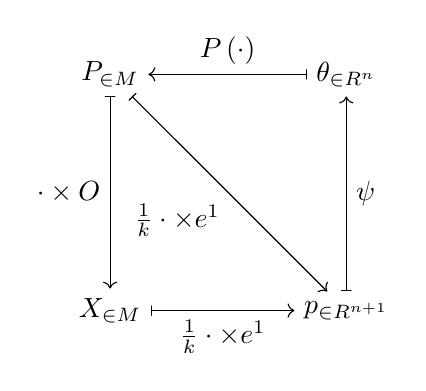
\begin{tikzpicture}
    \node (posit) at (0,0) {\(P_{\in M}\)};
    \node (point) at (0,-3) {\(X_{\in M}\)};
    \node (param) at (3,0) {\(\theta_{\in \mathbb{R}^n}\)};
    \node (vectr) at (3,-3) {\(p_{\in \mathbb{R}^{n+1}}\)};

    \draw[|->] (posit)--(point) node[midway,left] {\(\cdot\times O\)};
    \draw[|->] (point)--(vectr) node[midway,below] {\(\frac{1}{k}\cdot\times\tensor{e}{^1}\)};
    \draw[|->] (posit)--(vectr) node[midway,below left] {\(\frac{1}{k}\cdot\times\tensor{e}{^1}\)};
    \draw[|->] (param)--(posit) node[midway,above] {\(P\left(\cdot\right)\)};
    \draw[|->] (vectr)--(param) node[midway,right] {\(\psi\)};
\end{tikzpicture}
\end{document}